\documentclass[12pt]{article}

\usepackage{amsthm}
\usepackage{amsmath}
\usepackage{amsfonts}
\usepackage{mathrsfs}
\usepackage{amssymb}
\usepackage{units}
\usepackage{graphicx}
\usepackage{tikz-cd}
\usepackage{nicefrac}
\usepackage{hyperref}
\hypersetup{hidelinks}
\usepackage{bbm}
\usepackage{color}
\usepackage{tensor}
\usepackage{tipa}
\usepackage{bussproofs}
\usepackage{ stmaryrd }
\usepackage{ textcomp }
\usepackage{leftidx}
\usepackage{afterpage}

\newcommand\blankpage{
    \null
    \thispagestyle{empty}
    \addtocounter{page}{-1}
    \newpage
    }

\graphicspath{ {images/} }

\newtheorem{thm}{Theorem}
\newtheorem{defn}{Definition}
\newtheorem{lemma}{Lemma}
\newtheorem{example}{Example}
\newtheorem{notation}{Notation}
\newtheorem{cor}{Corollary}
\newtheorem{remark}{Remark}

\newcommand{\bb}[1]{\mathbb{#1}}
\newcommand{\scr}[1]{\mathscr{#1}}
\newcommand{\call}[1]{\mathcal{#1}}
\newcommand{\psheaf}{\text{\underline{Set}}^{\scr{C}^{\text{op}}}}
\newcommand{\und}[1]{\underline{\hspace{#1 cm}}}
\newcommand{\adj}[1]{\text{\textopencorner}{#1}\text{\textcorner}}

\usepackage[margin=3cm]{geometry}

\title{Approximation of Continuous Functions by ReLU Nets}
\author{Will Troiani}
\date{October 2019}

\begin{document}

\maketitle

\section{Introduction}
Feed-forward neural nets with a single hidden layer can approximate continuous functions on a compact domain if the hidden layer is allowed to be arbitrarily wide \cite{Cybenko}, \cite{Hornik}. Recently though \cite[\S 3]{Hanin17} there has been interest in feed-forward networks with bounded \emph{widths} rather than \emph{depth}. The goal of this note is to discuss the approximation of continuous functions on compact domains by ReLU nets with an upper bound on the widths (Theorem \ref{infinitecase} and Remark \ref{bound}). This work is based off \cite{Hanin}.

\section{Feed-forward Neural Nets, ReLU activations, and Max-min strings}
\begin{defn}
A \textbf{ReLU net} $\call{N}$ consists of
\begin{itemize}
    \item a (finite) sequence of \textbf{widths} $d_{in} = d_1,d_2,...,d_n = d_\text{out}$, where each $d_i \in \bb{N}$, $d_{\text{in}}$ is the \textbf{input width}, and $d_{\text{out}}$ the \textbf{output width},
    \item a sequence of affine functions $(A_i: \bb{R}^{d_i} \to \bb{R}^{d_{i+1}})_{i = 1}^{n-1}$,
\end{itemize}
\end{defn}
Associated to every ReLU net $\call{N}$ is a function
\begin{equation}
    f_{\call{N}}: A_n \text{ReLU}_{d_{n-1}} A_{n-1} ... \text{ReLU}_{d_1} A_1: \bb{R}^{d_{\text{in}}} \to \bb{R}^{d_{\text{out}}}
\end{equation}
where
\begin{align*}
    \text{ReLU}_k: \bb{R}^{k} &\to \bb{R}^k\\
    (x_1,...,x_k) &\mapsto \big(\operatorname{max}\lbrace 0,x_1\rbrace,...,\operatorname{max}\lbrace 0, x_k \rbrace\big)
\end{align*}
The subscript $k$ on ReLU$_k$ will be dropped when its value is clear from context.
The proof that ReLU nets can be used to approximate continuous functions with compact domains will not use ReLU nets on the nose, but instead will use functions which can be written as particular compositions involving affine functions as well as the $\operatorname{max}$ and $\operatorname{min}$ functions:
\begin{defn}
A \textbf{max-min string} is a function $g: \bb{R}^n \to \bb{R}^m$ which can be written as
\begin{equation}
    g = \sigma_{L-1}(l_L,\sigma_{L-2}(l_{L-1},...(\sigma_2(l_3,\sigma_1(l_2,l_1))...))
\end{equation}
where each $l_i: \bb{R}^n \to \bb{R}^m$ is an affine function, and each $\sigma_i$ is either the component-wise $\operatorname{max}$ function:
\begin{align*}
    \operatorname{max}: \bb{R}^{2m} &\to \bb{R}^m\\
    (x_1,...,x_m,y_1,...,y_m) &\mapsto (\operatorname{max}\lbrace x_1,y_1\rbrace,...,\operatorname{max}\lbrace x_m,y_m)
\end{align*}
or the component-wise $\operatorname{min}$ function:
\begin{align*}
    \operatorname{min}: \bb{R}^{2m} &\to \bb{R}^m\\
    (x_1,...,x_m,y_1,...,y_m) &\mapsto (\operatorname{min}\lbrace x_1,y_1\rbrace,...,\operatorname{min}\lbrace x_m,y_m\rbrace)
\end{align*}
\end{defn}
%
\begin{lemma}
\label{maxmin}
Let $g: \bb{R}^n \to \bb{R}^m$ a max-min string and $K \subseteq \bb{R}^n$ a compact set. Then there exists a ReLU net $\call{N}$ such that for all $x \in K$, $f_\call{N}(x) = g(x)$.
\end{lemma}
\begin{proof}
It can be assumed without loss of generality that $K$ lies in the positive orthant, that is,
\begin{equation*}
    K \subseteq \bb{R}_+^n := \lbrace (x_1,...,x_n) \in \bb{R}^n \mid 1 \leq i \leq n \Rightarrow x_i \geq 0 \rbrace
\end{equation*}
To see this, say that $K$ does \emph{not} lie in the positive orthant. Then let $T: K \to K'$ be a translation where $K'$ does lie in the positive orthant, such a translation exists as $K$ is compact. Then by the theorem (once it has been proved) there exists $\call{N}$ such that $f_\call{N} = gT^{-1}$, which implies $f_\call{N} T = g$, and $f_\call{N} T$ is a ReLU net.\\\\
%
So assume $K$ lies in the positive orthant and write $$g = \sigma_{L-1}(l_L,\sigma_{L-2}(l_{L-1},...(\sigma_2(l_3,\sigma_1(l_2,l_1))...))$$
where $l_i: \bb{R}^{n} \to \bb{R}^{m}$.\\\\
%
The key observation is that if $a,b \in \bb{R}$, then $\operatorname{max}\lbrace a,b\rbrace$ can be calculated by adding $a$ to $\operatorname{max}\lbrace 0, b - a\rbrace$, with a similar trick used for $\operatorname{min}$.\\\\
%
Define the following affine functions:
\begin{align*}
    A_1: \bb{R}^n &\to \bb{R}^m\\
    x &\mapsto (x,l_1(x))
\end{align*}
and if $i = 2,...,L$:
\begin{align*}
    A_i: \bb{R}^{n + m} &\to \bb{R}^{n + m}\\
    (x,y) &\mapsto 
    \begin{cases}
    (x, y - l_i(x))& \sigma_{i-1} = \operatorname{max}\\
    (x, -y + l_i(x))& \sigma_{i-1} = \operatorname{min}
    \end{cases}
\end{align*}
Notice that for $i = 2,...,L$, the functions $A_i$ admit inverses given by:
\begin{align*}
    A_i^{-1}: \bb{R}^{n + m} &\to \bb{R}^{n + m}\\
    (x,y) &\mapsto 
    \begin{cases}
    (x, y + l_i(x))& \sigma_{i-1} = \operatorname{max}\\
    (x, -y + l_i(x))& \sigma_{i-1} = \operatorname{min}
    \end{cases}
\end{align*}
Then the function
\[h := \text{ReLU}\text{ }A_{L}^{-1}\text{ }\text{ReLU}\text{ }A_L\text{ }...\text{ }A_1^{-1}\text{ }\text{ReLU}\text{ }A_1\]
is equal to the graph of $g$. Thus $\pi h = g$, where $\pi: \bb{R}^{2m} \to \bb{R}^m$ is the map $(x_1,...,x_n,y_1,...,y_m) \mapsto (y_1,...,y_m)$, and $\pi h$ is a ReLU net.
\end{proof}

\section{Approximation of Continuous Functions by ReLU Nets, Finite Case}
It follows from Lemma \ref{maxmin} that in order to approximate a continuous function $f: K \to \bb{R}^m$ using a ReLU net, it suffices to approximate $f$ with a max-min string. The goal of section \ref{main} below is to show how this can be done. The proof will require some technical analysis, but the broad idea is highlighted well by considering the case when $K$ is a finite set. In fact, in the finite case, $f$ can be computed exactly using a ReLU net:
\begin{lemma}
\label{finitecase}
Let $\epsilon \in \bb{R}_{>0}$ and $f: S \to \bb{R}^m$ a function with $S$ finite. Then there exists a max-min string $g: \bb{R}^n \to \bb{R}^m$ such that $f = g$.
\end{lemma}
The following Lemma will be used:
\begin{lemma}
\label{bigaffinefunctionfinite}
Let $f: S \to \bb{R}^m$ be a function with $S \subseteq \bb{R}^n$ a finite set. For any $t \in \bb{R}_{\geq 0}$ and any $x \in \bb{R}\setminus S$ there exists an affine function $l = (l_1,...,l_m): \bb{R}^n \to \bb{R}^m$ such that
\begin{itemize}
    \item $l(x) = (0,...,0)$,
    \item $t < l_i(s)$ for all $s \in S$
\end{itemize}
\end{lemma}
\begin{proof}
Many such functions $l$ can be defined, but in order to reflect the construction which will be used to prove the case where $S$ is an arbitrary compact set, the case when $n = 2$ and $m = 1$ will be considered and a particular construction will be shown which perhaps is not the most obvious one.\\\\
%
Let $A,B \in \bb{R}^2$ be points such that $\Delta AxB$ forms a triangle, $S\cap \Delta AxB = \lbrace x \rbrace$ and $S$ lies in the infinite planar sector $\angle AxB$, ie
\[S \subseteq \angle AxB := \lbrace \big(\gamma_1(B - x),\gamma_2(C - x)\big) \mid \gamma_1,\gamma_2 \geq 0\rbrace\]
see figure \ref{infiniteplanarsector}.
\begin{figure}
    \centering
    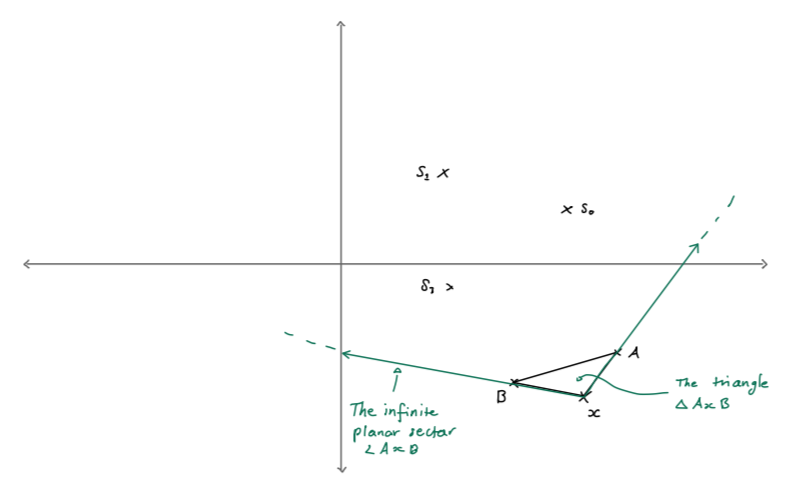
\includegraphics[width = \textwidth]{Sections/Diagrams/infiniteplanarsector.png}
    \caption{An example of an appropriate choice of triangle for the proof of Lemma \ref{bigaffinefunctionfinite}.}
    \label{infiniteplanarsector}
\end{figure}
Then let $l$ be the affine function such that $l(x) = 0$ and $l(A) = l(B) = t$. See figure \ref{bigaffinefinitezero}
\begin{figure}
    \centering
    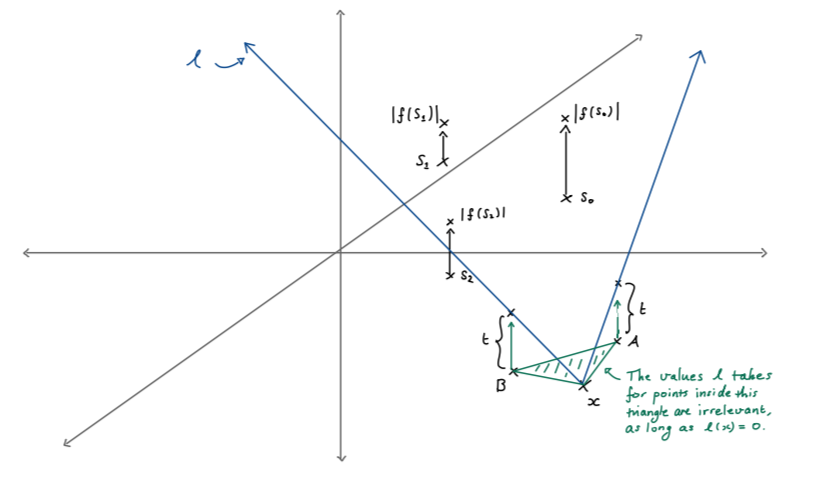
\includegraphics[width=\textwidth]{Sections/Diagrams/bigaffinefinite.png}
    \caption{The affine function $l$.}
    \label{bigaffinefinitezero}
\end{figure}
\end{proof}
%
\begin{proof}[Proof of Lemma \ref{finitecase}]
If $S = \lbrace s \rbrace$ contains a single element, then the max-min string $g(s) = f(s)$ can be used. So say $S$ contains at least two elements. Fix an element $s \in S$ and let $g: S\setminus\lbrace s \rbrace \to \bb{R}^m$ be a max-min string satisfying $\forall s' \in S\setminus\lbrace s\rbrace$, $g(s') = f(s')$. Set 
\[t = \operatorname{max}_{s' \in S \setminus \lbrace s \rbrace}\lbrace |g(s') - f(s)|\rbrace\]
and let $l = (l_1,...,l_m): \bb{R}^n \to \bb{R}^m$ be an affine function such that $l(s) = 0$ and for all $s' \in S \setminus \lbrace s \rbrace$, $l_i(s') > t$, which exists by Lemma \ref{bigaffinefunctionfinite}. Write $f = (f_1,...,f_m)$, then 
\begin{equation}
\label{lboundfinite}
\forall s' \in S\setminus\lbrace s \rbrace,\forall i = 1,...,m,\qquad f_i(s) - l_i(s') < g_i(s') < f_i(s) + l_i(s')
\end{equation}
Define the max-min string:
\[\hat{g} = \operatorname{max}\lbrace \operatorname{min}\lbrace g, f(s) + l\rbrace, f(s) - l\rbrace\]
which is such that $\hat{g}(s') = f(s')$ for all $s' \in S$. Indeed,
\begin{align*}
    \hat{g}(s) &= \operatorname{max}\lbrace \operatorname{min}\lbrace g(s), f(s) + l(s)\rbrace, f(s) - l(s)\rbrace\\
    &= \operatorname{max}\lbrace \operatorname{min}\lbrace g(s), f(s)\rbrace, f(s)\rbrace\\
    &= f(s)
\end{align*}
and if $s' \in S\setminus \lbrace s \rbrace$,
\begin{align*}
    \hat{g}(s') &= \operatorname{max}\lbrace \operatorname{min}\lbrace g(s'), f(s) + l(s')\rbrace, f(s) - l(s')\rbrace\\
    &= \operatorname{max}\lbrace g(s'), f(s) - l(s')\rbrace\\
    &= g(s') = f(s')
\end{align*}
where the first and second equality follow from \ref{lboundfinite}.
\end{proof}

\section{Approximation of Continuous Functions by ReLU Nets, General Case}
\label{main}
The goal of this section is to prove that ReLU nets can approximate continuous functions $f: K \to \bb{R}$, where $K$ is compact (for a formal statement see Theorem \ref{infinitecase} below). This will be done by approximating a continuous function $f: \bb{R}^2 \to \bb{R}$ on a compact subset $K \subseteq \bb{R}^2$. Again, a ReLU net which approximates $f$ itself will not be directly constructed, but a max-min string will be instead, which is sufficient by Lemma \ref{maxmin}.\\\\
%
In the finite case, a max-min string $g: S\setminus\lbrace s \rbrace \to \bb{R}^m$ was extended to $\hat{g}: S \to \bb{R}^m$. The existence of $\hat{g}$ used crucially that there existed an affine function $l: \bb{R}^n \to \bb{R}^m$ such that each entry of $l(s')$ was larger than the corresponding entry of $g(s')$, for all $s' \in S\setminus\lbrace s \rbrace$, and was such that $l(s) = 0$. The key realisation in the case where $K$ is an arbitrary compact set is the existence of an analogous affine function $l$:
%
\begin{defn}
The \textbf{inverse modulus of continuity of $\epsilon$} of a continuous function $f: \bb{R}^2 \to \bb{R}$ in the domain $K \subseteq \bb{R}^2$ is
\[w_{f,K}^{-1}(\epsilon) = \operatorname{sup}\lbrace \delta \in \bb{R} \mid \forall x, y \in K\text{, }|x - y| \leq \delta \Rightarrow |f(x) - f(y)| \leq \epsilon\rbrace\]
\end{defn}
%
%
%
%
%
%
%
%
%
%
\begin{lemma}
\label{circlelemma}
Let $f: \bb{R}^2 \to \bb{R}$ be continuous, $\epsilon > 0$, $r > r' > 0$. Let $S_r := \lbrace (x,y) \in \bb{R}^2 \mid x^2 + y^2 = r \rbrace$ be the circle of radius $r$. Let $X,Y \in S_r$ be such that $|X - Y| \leq r$ and $X',Y' \in S_{r'}$ be such that $X',X,Y,Y'$ are collinear, and let $Z \in S_{r'}$ be the point on the arc connecting $X'$ to $Y'$ and the straight line which passes through the origin and the midpoint of the straight line connecting $X$ and $Y$. See Figure \ref{elelprime}.
\begin{figure}[h]
    \centering
    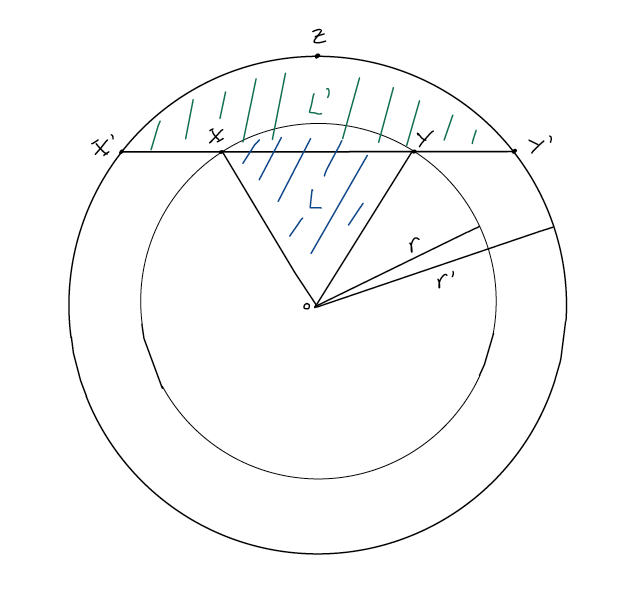
\includegraphics[width=20em]{Sections/Diagrams/elelprime.png}
    \caption{The configuration described in Lemma \ref{circlelemma}}
    \label{elelprime}
\end{figure}
Let $L$ denote the minor sector of $S_r$ induced by the radii $0X$ and $0Y$ and let $L'$ denote the minor segment of $S_{r'}$ induced by the chord which connects $X'$ to $Y'$. If
\[\operatorname{Diam}(L') \leq w_{f,B_{r'}(0)}^{-1}(\epsilon)\]
then there exists an affine function $l: \bb{R}^2 \to \bb{R}$ such that
\begin{itemize}
    \item $l(x) \leq \epsilon$ for all $x \in L'$,
    \item $|f(x) - f(Z)| \leq l(x) + \epsilon$ for all $x \in L$.
\end{itemize}
\end{lemma}
%
%
%
%
%
%
%
%
%
%
%
\begin{proof}
Let $l$ be the affine function such that $l(Z) = 0$ and $l(X') = l(Y') = \epsilon$. Let $x \in L$. Denote by $Z' \in \bb{R}^2$ the point which is collinear to $X',Y',X,Y$ and is also collinear to $Z,x$. Then as $l$ is affine and $|x - Z| \leq |Z' - Z|$, it follows that $l(x) \leq l(Z') = \epsilon$.\\\\
%
Say $x \in L'$. Then write $|x - Z| = kw_{f,B_{r'}(0)}^{-1}(\epsilon) + \rho$ where $k \in \bb{N}$ and $0 \leq \rho < w_{f,B_{r'}(0)}^{-1}(\epsilon)$. Then
\begin{align*}
    &|x - Z| = kw_{f,B_{r'}(0)}^{-1}(\epsilon) + \rho\\
    &\Rightarrow |x - Z| \geq kw_{f,B_{r'}(0)}^{-1}(\epsilon)\\
\end{align*}
and so,
\begin{equation}
\label{integerandremainder}
    \frac{\epsilon |Z - x|}{w_{f,B_{r'}(0)}^{-1}(\epsilon)} \geq k\epsilon
\end{equation}
Also, consider a sequence of points $Z = x_1,x_2,...,x_{k+1} = x$ such that $|x_{i+1} - x_i| = w_{f,B_{r'}(0)}^{-1}(\epsilon)$ for $i = 1,...,k-1$ and $|x_{k+1} - x_k| < w_{f,B_{r'}(0)}^{-1}(\epsilon)$. See Figure \ref{devastation}.
\begin{figure}
    \centering
    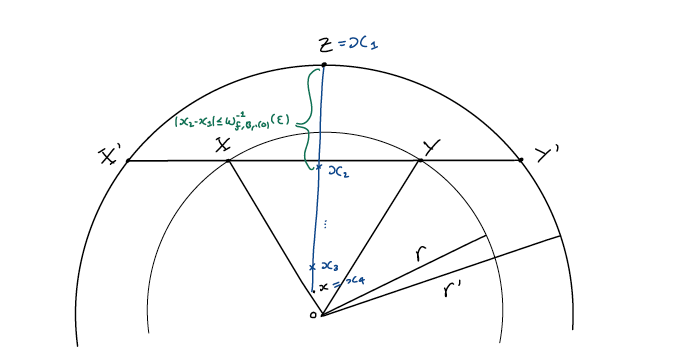
\includegraphics[width = 40em]{Sections/Diagrams/devastation.png}
    \caption{The points $x_1,...,x_n$ in the proof of Lemma \ref{circlelemma}}
    \label{devastation}
\end{figure}Then
\begin{align*}
    |f(x) - f(Z)| &= |f(x_1) - f(x_2) + f(x_2) - f(x_3) + ... + f(x_2) - f(x_1)|\\
    &\leq |f(x_1) - f(x_2)| + ... + |f(x_2) - f(x_1)|\\
    &< k\epsilon + \epsilon
\end{align*}
and so,
\begin{equation}
    \label{triangleineq}
    |f(x) - f(Z)| < k\epsilon + \epsilon
\end{equation}
Equations \ref{integerandremainder} and \ref{triangleineq} together imply
\[|f(x) - f(Z)| < \frac{\epsilon |x - Z|}{w_{f,B_{r'}(0)}^{-1}(\epsilon)} + \epsilon\]
Thus it remains to show:
\[\frac{\epsilon |x - Z|}{w_{f,B_{r'}(0)}^{-1}(\epsilon)} \leq l(x)\]
This comes down to the fact that the slope of $l$ in the direction of the vector $x - Z$ can be bounded below by $\frac{\epsilon}{w_{f,B_{r'}(0)}^{-1}(\epsilon)}$. More precisely, consider the following parametrisation of the straight line which intersects $Z$ and $x$:
\begin{align*}
    c: \bb{R} &\to \bb{R}^2\\
    s &\mapsto Z + \frac{s}{|x - Z|}(x - Z)
\end{align*}
Then the function $lc: \bb{R} \to \bb{R}$ is affine, and in fact is linear as
\[lc(0) = l(Z) = 0\]
So for all $y \in \bb{R}$, $lc(y) = my$ for some gradient $m$. Let $W \in \bb{R}^2$ be the point which intersects the line parametrised by $c$ and the line which passes through $X$ and $Y$. Then since $|W - Z| \leq w_{f,B_{r'}(0)}^{-1}(\epsilon)$ and $l(W) = \epsilon$, it follows that:
\[m = \frac{l(W) - l(Z)}{|W - Z|} = \frac{\epsilon}{|W - Z|} \geq \frac{\epsilon}{w_{f,B_{r'}(0)}^{-1}(\epsilon)}\]
and so:
\[\frac{\epsilon |x - Z|}{w_{f,B_{r'}(0)}^{-1}(\epsilon)} \leq m|x - Z| = lc(|x - Z|) = l(x)\]
which completes the proof.
\end{proof}
%
%
%
%
%
%
%
%
%
%
%
\begin{cor}
\label{cor:geometric-maxmin}
In the setting of Lemma \ref{circlelemma}, but with every instance of $\epsilon$ replaced by $\frac{\epsilon}{2}$, if there exists a max-min string $g: \bb{R}^2 \to \bb{R}$ which approximates $f$ on $L'$ then there exists a max-min string $\hat{g}: \bb{R}^2 \to \bb{R}$ which approximates $f$ on $L \cup L'$.
\end{cor}
%
%
%
%
%
%
%
%
%
%
%
\begin{proof}
Let $l: \bb{R}^2 \to \bb{R}$ be an affine function such that
\begin{itemize}
    \item $l(x) \leq \frac{\epsilon}{2}$, for all $x \in L'$,
    \item $|f(x) - f(Z)| \leq l(x) + \frac{\epsilon}{2}$, for all $x \in L$
\end{itemize}
the existence of which is guaranteed by Lemma \ref{ballapprox}. Then define the max-min string
\[\hat{g} = \operatorname{max}\lbrace \operatorname{min}\lbrace g, f(Z) + l\rbrace, f(Z) - l\rbrace\]
On $L$, we have $f \leq g + \epsilon$ and
\[f\leq f(Z) + l + \epsilon\]
so
\begin{align*}
    f &\leq \operatorname{min}\lbrace g + \epsilon, f(Z) + l + \epsilon\rbrace\\
    &= \operatorname{min}\lbrace g, f(Z) + l\rbrace + \epsilon\\
    &\leq \operatorname{max}\big\lbrace\operatorname{min}\lbrace g, f(Z) + l \rbrace, f(Z) - l\big\rbrace + \epsilon\\
    &= \hat{g} + \epsilon
\end{align*}
Similarly, since $g - \epsilon \leq f$ and
\[f(Z) - l - \epsilon \leq f\]
it follows that
\begin{align*}
    \hat{g} - \epsilon &= \operatorname{max}\big\lbrace \operatorname{min}\lbrace g, f(Z) + l - \epsilon\rbrace, f(Z) - l\big\rbrace - \epsilon\\
    &= \operatorname{max}\lbrace \operatorname{min}\lbrace g - \epsilon, f(Z) + l - \epsilon\rbrace, f(Z) - l - \epsilon\rbrace\\
    &\leq \operatorname{max}\lbrace g - \epsilon, f(Z) - l - \epsilon\rbrace\\
    &\leq f
\end{align*}
On $L'$, by construction:
\[f(Z) - \frac{\epsilon}{2} \leq f(Z) - l \leq \hat{g} \leq f(Z) + l \leq f(Z) + \frac{\epsilon}{2}\]
and for all $x \in L'$
\[|f(x) - f(Z)| \leq \frac{\epsilon}{2}\]
by definition of $w_{f,B_{r'}(0)}^{-1}(\frac{\epsilon}{2})$. Thus:
\begin{align*}
    |\hat{g}(x) - f(x)| &= |\hat{g}(x) - f(Z) + f(Z) - f(x)|\\
    &\leq |\hat{g}(x) - f(Z)| + |f(Z) - f(x)|\\
    &\leq \frac{\epsilon}{2} + \frac{\epsilon}{2}\\
    &= \epsilon
\end{align*}
%
\end{proof}
%
%
%
%
%
%
%
%
%
%
%
Next we turn to two geometric Lemmas:%
%
%
%
%
%
%
%
%
%
%
%
\begin{lemma}
\label{elementarygeometryone}
Consider two concentric circles, $S_R$ and $S_{R'}$ with $R' > R$. Consider a chord intersecting points $X$ and $Y$ on $S_R$ and extend this chord so that it intercepts $S_{R'}$, at $X'$ and $Y'$ say (see Figure \ref{fig:elementarygeometryone}). Then
\[|X'Y'|^2 = 4(R'^2 - R^2) + |XY|^2\]
\end{lemma}
\begin{proof}
Let $P$ denote the midpoint of the line $XY$. Then $|P| = \sqrt{R^2 - \frac{1}{4}|XY|^2}$ (again, see Figure \ref{fig:elementarygeometryone}).
\begin{figure}
    \centering
    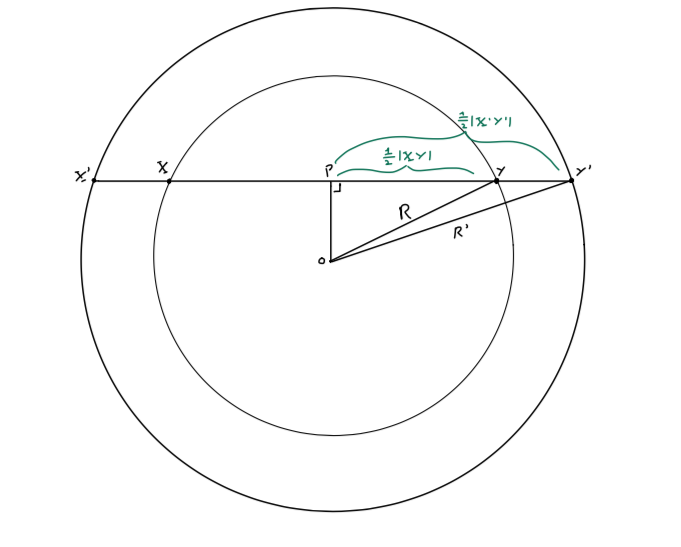
\includegraphics[width = 25em]{Sections/Diagrams/elementarygeometry.png}
    \caption{The geometry of Lemma \ref{elementarygeometryone}}
    \label{fig:elementarygeometryone}
\end{figure}
Thus
\begin{equation*}
    \Big(\sqrt{R^2 - \frac{1}{4}|XY|^2}\Big)^2 + \frac{1}{4}|X'Y'|^2 = R'^2
\end{equation*}
from which, the result follows.
\end{proof}
%
%
%
%
%
%
%
%
%
%
\begin{lemma}
\label{elementarygeometrytwo}
Let $X,Y$ be points on $S_R$ such that $0 < |X - Y| \leq R$. Let $\tau_X$ and $\tau_Y$ be straight lines tangent to $S_R$ respectively at $X$ and $Y$. Let $T$ denote the intersection of $\tau_X$ and $\tau_Y$. Then $\operatorname{Diam}(\Delta XTY) = |X - Y|$
\end{lemma}
%
%
%
%
%
%
%
%
%
%
\begin{proof}
If $|X - Y| = R$ then the triangle $XOY$ is equilateral. It follows from this that angle $\angle TXY$ and $\angle TYX$ are both equal to $30^\circ$. As $|X - Y|$ decreases, both angles $\angle TXY$ and $\angle TYX$ decrease. So if $|X - Y| \leq R$ the angle $\angle XTY$ is obtuse, which implies that $\operatorname{Diam}(\Delta XTY) = |X - Y|$. See Figure \ref{fig:elementarygeometrytwo}.
\begin{figure}
    \centering
    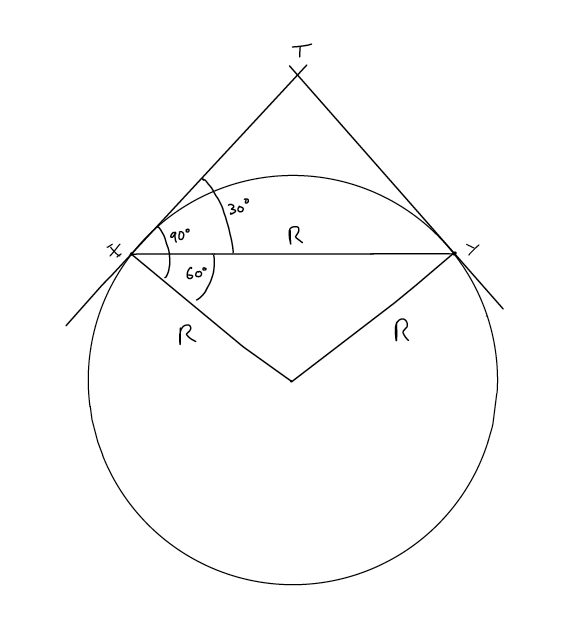
\includegraphics[width = 20em]{Sections/Diagrams/elementarygeomtwo.png}
    \caption{The geometry of Lemma \ref{elementarygeometrytwo}}
    \label{fig:elementarygeometrytwo}
\end{figure}
\end{proof}
%
%
%
%
%
%
%
%
%
%
%
\begin{lemma}
\label{ballapprox}
Let $f: \bb{R}^2 \to \bb{R}$ be continuous, $\epsilon > 0$, $R > 0$. Assume $w_{f,B_{R}(0)}^{-1}(\frac{\epsilon}{2})$ and let $R' > w_{f,B_{R}(0)}^{-1}(\frac{\epsilon}{2})$. Assume further that there exists a max-min string $g: \bb{R}^2 \to \bb{R}$ which approximates $f$ on $B_{R'}(0)$. Let $R''$ be
\[R'' := \sqrt{R'^2 + \frac{w_{f,B_{R}(0)}^{-1}(\frac{\epsilon}{2})}{\sqrt{2}R'}}\] If $R'' < R$ then there exists a max-min string $\hat{g}: \bb{R}^2 \to \bb{R}$ which approximates $f$ on $B_{R''}(0)$, and if $R'' \geq R$ then there exists a max-min string $\hat{g}: \bb{R}^2 \to \bb{R}$ which approximates $f$ on $B_{R}(0)$.
\end{lemma}
%
%
%
%
%
%
%
%
%
%
\begin{proof}
To ease notation let $a_{R'} := \frac{w_{f,B_{R}(0)}^{-1}(\frac{\epsilon}{2})}{\sqrt{2}R'}$. Let $X,Y \in \bb{R}^2$ lie on the circle of radius $R'$ which satisfy
\[|XY| = w_{f,B_{R}(0)}^{-1}(\frac{\epsilon}{2})(1 - a_{R'})^{\frac{1}{2}}\]
such a pair $(X,Y)$ exists as
\[|XY|^2 = w_{f,B_{R}(0)}^{-1}(\frac{\epsilon}{2})^2(1 - a_{R'}^2) < w_{f,B_{R}(0)}^{-1}(\frac{\epsilon}{2}) \leq R'\]
We consider first the case when $R'' < R$. Let $X',Y' \in \bb{R}^2$ lie on the circle of radius $R''$ which intersect the line segment connecting $X$ and $Y$. Let $L$ denote the minor segment on the circle of radius $R'$ induced by the chord which connects $X'$ to $Y'$ and let $L'$ denote the minor sector on the circle of radius $R'$ induced by the radii $0X$ and $0Y$. Let $Z$ denote the intersection of the circle of radius $R''$ and the line which connects $0$ and the midpoint of the line $XY$. See Figure \ref{ballconfig}.
\begin{figure}
    \centering
    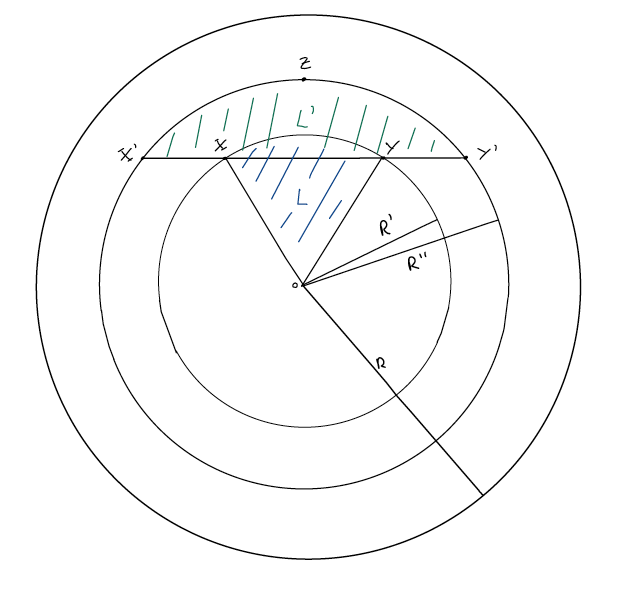
\includegraphics[width=20em]{Sections/Diagrams/ballconfig.png}
    \caption{Configuration of the balls in Lemma \ref{ballapprox}}
    \label{ballconfig}
\end{figure}
By Lemma \ref{elementarygeometryone} and a direct calculation,
\[|X'Y'| = \sqrt{4(R^{''2} - R^{'2}) + |XY|^2} = w_{f,B_{R}(0)}^{-1}(\frac{\epsilon}{2})\]
Moreover, $w_{f,B_{R}(0)}^{-1}(\frac{\epsilon}{2}) < R' < R''$, so by Lemma \ref{elementarygeometrytwo}:
\[\operatorname{Diam}(L) \leq w_{f,B_{R}(0)}^{-1}(\frac{\epsilon}{2})\]
Thus the hypotheses of Corollary \ref{cor:geometric-maxmin} are satisfied.\\\\
%
The case when $R'' \geq R$ is almost identical but the pair $(X',Y')$ are taken to intersect the ball of radius $R$ instead of the ball of radius $R''$.
\end{proof}
%
%
%
%
%
%
%
%
%
%
%
This brings us to the main Theorem:
\begin{thm}
\label{infinitecase}
Let $\epsilon \in \bb{R}_{>0}$ and $f: \bb{R}^2 \to \bb{R}$ be continuous, and $K \subseteq \bb{R}^2$ compact. Then there exists a max-min string $g: \bb{R}^2 \to \bb{R}$ such that
\[\forall x \in K,\text{ }|g(x) - f(x)| \leq \epsilon\]
\end{thm}
\begin{proof}
Since compact subsets of $\bb{R}^2$ are bounded, it suffices to consider the case when $K = B_R := \lbrace x \in \bb{R}^2 \mid |x| \leq R\rbrace$, for some $R \in \bb{R}$. If $R \leq w_{f,B_{R}(0)}^{-1}\big(\frac{\epsilon}{2}\big)$ then the max-min string $g: \bb{R}^2 \to \bb{R}$ which is the constant function $g \equiv f(0)$ suffices. Suppose $w_{f,B_{R}(0)}^{-1}\big(\frac{\epsilon}{2}\big) < R$ and $f: B_R(0) \to \bb{R}$ are given. Consider the following set
\[\scr{X} := \lbrace R' \in \bb{R} \mid \text{there exists a max-min string } g\text{ which approximates }f\text{ on }B_{R}(0)\rbrace\]
We claim that $R \in \scr{X}$, recall the notation from Lemma \ref{ballapprox} that $a_R := \frac{w_f^{-1}\big(\frac{\epsilon}{2}\big)^2}{\sqrt{2}R}$. Suppose for a contradiction that $R \not\in \scr{X}$, then $\scr{X}$ is bounded above. Let $s^2 = \sup\scr{X}^2$ and $R' \in \scr{X}$ to be such that
\[s^2 - a_s < R'^2\]
Notice that $s \not\in \scr{X}$ as if $s \in \scr{X}$ then Lemma \ref{ballapprox} can be used to find a strictly greater value in $\scr{X}$. As $R' < s$, it follows that $a_s < a_{R'}$ and
\[s^2 < R'^2 + a_s < R'^2 + a_{R'}\]
thus
\[s < \sqrt{R'^2 + a_{R'}}\]
but by Lemma \ref{ballapprox}, $\sqrt{R'^2 + a_{R'}} \in \scr{X}$, contradicting that $s$ is a supremum.
\end{proof}

\begin{remark}
\label{bound}
As mentioned earlier, Theorem \ref{infinitecase} generalises to continuous functions $f: K \to \bb{R}^m$ where $K \subseteq \bb{R}^n$. Ie, given $\epsilon > 0$ there exists a max-min string $g: \bb{R}^n \to \bb{R}^m$ such that for all $x \in K$,
\[|f(x) - g(x)| < \epsilon\]
Lemma \ref{maxmin} then implies that there exists a ReLU net with input width $n$ and all other widths equal to $n + m$ which approximates $f$. This gives the promised upper bound on the widths. In fact a lower bound can be proved as well, see \cite[\S 3]{Hanin}.
\end{remark}

\section{AI-powered addendum}
\label{sec:ai-powered-addendum}

This addendum records the mathematical corrections to the preceding notes and gives replacement statements which can be used without relying on the informal geometric sketches.  The original goal is correct: continuous functions on compact sets can be uniformly approximated by ReLU networks.  Several intermediate lemmas in the notes, however, are false as stated or have hypotheses, dimensions, or regions interchanged.  The safest repair is to replace the circle-growth proof by the explicit max-min construction below.

\subsection{Corrected definitions}

\begin{defn}[ReLU network, corrected]
Let $\rho(t)=\max\{0,t\}$ and let $\rho_d:\bb{R}^d\to\bb{R}^d$ denote the component-wise ReLU map.  A feed-forward ReLU network with input dimension $d_0$ and output dimension $d_L$ consists of affine maps
\[
A_i:\bb{R}^{d_{i-1}}\longrightarrow \bb{R}^{d_i},\qquad i=1,\ldots,L,
\]
where $d_1,\ldots,d_{L-1}$ are the hidden widths.  Its realised function is
\[
f_{\call N}=A_L\circ \rho_{d_{L-1}}\circ A_{L-1}\circ\cdots\circ \rho_{d_1}\circ A_1.
\]
Thus the last affine map is not followed by a ReLU unless this is explicitly declared.
\end{defn}

\begin{remark}[Indexing error in the original definition]
The displayed expression
\[
A_n\operatorname{ReLU}_{d_{n-1}}A_{n-1}\cdots \operatorname{ReLU}_{d_1}A_1
\]
uses an affine map $A_n$ that was not included in the preceding list of affine maps.  The corrected indexing is the one in the previous definition.
\end{remark}

\begin{defn}[Max-min strings, corrected]
For affine maps $l_1,\ldots,l_N:\bb{R}^n\to\bb{R}^m$, a max-min string is any function obtained from the $l_i$ by finitely many component-wise operations
\[
(u,v)\longmapsto u\vee v,
\qquad
(u,v)\longmapsto u\wedge v,
\]
where
\[
(u\vee v)_j=\max\{u_j,v_j\},
\qquad
(u\wedge v)_j=\min\{u_j,v_j\}.
\]
Equivalently, after ordering the affine maps appropriately, one can write
\[
h_1=l_1,
\qquad
h_{i+1}=h_i\vee l_{i+1}\quad\text{or}\quad h_{i+1}=h_i\wedge l_{i+1},
\qquad
g=h_N.
\]
\end{defn}

\subsection{Max-min strings and ReLU networks}

\begin{lemma}[Realising max and min with ReLU]
For scalar inputs,
\[
\max\{a,b\}=b+\rho(a-b),
\qquad
\min\{a,b\}=a-\rho(a-b).
\]
The same identities hold component-wise on $\bb{R}^m$.
\end{lemma}

\begin{proof}
If $a\geq b$, then $\rho(a-b)=a-b$, so the two formulas give $a$ and $b$.  If $a<b$, then $\rho(a-b)=0$, so the two formulas give $b$ and $a$.
\end{proof}

\begin{lemma}[Correct replacement for Lemma \ref{maxmin}]
\label{ai:maxmin_relu}
Let $K\subseteq\bb{R}^n$ be compact and let $g:\bb{R}^n\to\bb{R}^m$ be a max-min string.  Then there is a ReLU network $\call N$ whose realised function agrees with $g$ on $K$.  The construction may be made with hidden widths $n+m$.
\end{lemma}

\begin{proof}
Write $g$ using affine maps $l_1,\ldots,l_N:\bb{R}^n\to\bb{R}^m$.  Choose $b\in\bb{R}^n$ such that
\[
x+b\in\bb{R}^n_{\geq0}\qquad\text{for all }x\in K.
\]
Because $K$ is compact and only finitely many affine functions are involved, choose $C>0$ such that
\[
l_i(x)+C\mathbf 1_m\in\bb{R}^m_{\geq0}
\qquad\text{for all }x\in K\text{ and all }i,
\]
where $\mathbf 1_m=(1,\ldots,1)$.  Work with the shifted variables
\[
u=x+b,
\qquad
L_i(u)=l_i(u-b)+C\mathbf 1_m.
\]
The shifted string $g+C\mathbf 1_m$ is obtained from the nonnegative affine functions $L_i$ by the same sequence of max and min operations.

At any intermediate stage store a pair $(u,y)\in\bb{R}^n\times\bb{R}^m$ with $u\geq0$ and $y\geq0$ on $K$.  To replace $y$ by $y\vee L_i(u)$, use the affine maps
\[
B_i(u,y)=(u,y-L_i(u)),
\qquad
B_i^{-1}(u,z)=(u,z+L_i(u)).
\]
Since $u\geq0$, the ReLU map leaves the $u$-coordinates unchanged, and
\[
B_i^{-1}\rho_{n+m}B_i(u,y)
=(u,\rho_m(y-L_i(u))+L_i(u))
=(u,y\vee L_i(u)).
\]
To replace $y$ by $y\wedge L_i(u)$, use
\[
C_i(u,y)=(u,L_i(u)-y),
\qquad
C_i^{-1}(u,z)=(u,L_i(u)-z),
\]
which gives
\[
C_i^{-1}\rho_{n+m}C_i(u,y)
=(u,L_i(u)-\rho_m(L_i(u)-y))
=(u,y\wedge L_i(u)).
\]
Begin with the affine map
\[
x\longmapsto (x+b,l_1(x)+C\mathbf 1_m).
\]
The first ReLU does nothing on $K$.  Iterating the blocks above produces $(x+b,g(x)+C\mathbf 1_m)$ on $K$.  The final affine map $(u,y)\mapsto y-C\mathbf 1_m$ gives $g(x)$.  Consecutive affine maps may be combined, so this is a feed-forward ReLU network in the standard sense.
\end{proof}

\begin{remark}[What was wrong in the original proof]
The map labelled $A_1$ in the original proof has the wrong codomain: $x\mapsto (x,l_1(x))$ takes values in $\bb{R}^{n+m}$, not in $\bb{R}^m$.  Moreover, $A_1^{-1}$ is not defined, because $A_1:\bb{R}^n\to\bb{R}^{n+m}$ is not invertible.  Finally, the proof assumes that arbitrary affine outputs survive ReLU unchanged; this is only true after a positivity shift on the compact set, or after encoding signed quantities by positive and negative parts.
\end{remark}

\subsection{Finite interpolation}

\begin{remark}[The affine separation lemma is false as stated]
Lemma \ref{bigaffinefunctionfinite} is false without an additional separation hypothesis.  In $\bb{R}$, take
\[
S=\{-1,1\},
\qquad
x=0,
\]
and ask for an affine function $l(t)=at+b$ with $l(0)=0$ and $l(-1)>0$, $l(1)>0$.  Then $b=0$, so the inequalities become $-a>0$ and $a>0$, impossible.

The statement becomes true if $x$ is an exposed point of $\operatorname{conv}(S\cup\{x\})$.  Equivalently, if there is a linear functional $\lambda$ with $\lambda(s-x)>0$ for all $s\in S$, then for any $t\geq0$ the affine function
\[
l(y)=c\lambda(y-x)
\]
with $c$ sufficiently large satisfies $l(x)=0$ and $l(s)>t$ for all $s\in S$.
\end{remark}

\begin{lemma}[Finite interpolation, corrected]
\label{ai:finite_interpolation}
Let $S\subseteq\bb{R}^n$ be finite and let $f:S\to\bb{R}^m$ be any function.  Then there is a max-min string $g:\bb{R}^n\to\bb{R}^m$ such that
\[
g(s)=f(s)\qquad\text{for every }s\in S.
\]
\end{lemma}

\begin{proof}
If $S$ has one point, take $g$ to be the corresponding constant affine map.  Otherwise, for each $s\in S$ choose $M_s>0$ so large that, for every $t\in S\setminus\{s\}$ and every component $j=1,\ldots,m$,
\[
f_j(s)-M_s\lVert t-s\rVert_\infty < f_j(t).
\]
This is possible because $S$ is finite and $\lVert t-s\rVert_\infty>0$ for $t\neq s$.  Define
\[
q_s(x)=f(s)-M_s\lVert x-s\rVert_\infty\mathbf 1_m.
\]
The scalar function $-\lVert x-s\rVert_\infty$ is a finite minimum of affine functions:
\[
-\lVert x-s\rVert_\infty
=\bigwedge_{i=1}^n\big((x_i-s_i)\wedge(s_i-x_i)\big).
\]
Hence each $q_s$ is a max-min string.  Now set
\[
g(x)=\bigvee_{s\in S}q_s(x),
\]
where the maximum is taken component-wise.  At a point $t\in S$, the term $q_t(t)$ equals $f(t)$, while $q_s(t)<f(t)$ component-wise for every $s\neq t$.  Thus $g(t)=f(t)$.
\end{proof}

\begin{remark}[Edits to Lemma \ref{finitecase}]
The parameter $\epsilon$ is unused in Lemma \ref{finitecase}.  The conclusion should not be written as $f=g$, because $f$ has domain $S$ while $g$ has domain $\bb{R}^n$.  The corrected conclusion is
\[
g(s)=f(s)\qquad\text{for all }s\in S.
\]
In the proof, the inductive hypothesis should produce a max-min string on $\bb{R}^n$ agreeing with $f$ on $S\setminus\{s\}$, not a function whose domain is only $S\setminus\{s\}$.
\end{remark}

\subsection{A clean replacement for the general approximation proof}

The geometric ball-expansion proof in Section \ref{main} can be replaced by the following direct max-min construction.  It proves the natural $\bb{R}^n\to\bb{R}^m$ statement and does not require extending $f$ off $K$.

\begin{thm}[Uniform approximation by max-min strings, corrected]
\label{ai:uniform_approximation}
Let $K\subseteq\bb{R}^n$ be compact and let $f:K\to\bb{R}^m$ be continuous.  For every $\epsilon>0$ there exists a max-min string $g:\bb{R}^n\to\bb{R}^m$ such that
\[
\sup_{x\in K}\lVert g(x)-f(x)\rVert_\infty\leq \epsilon.
\]
Consequently, by Lemma \ref{ai:maxmin_relu}, there exists a ReLU network whose realised function approximates $f$ to within $\epsilon$ on $K$.
\end{thm}

\begin{proof}
Since $K$ is compact, $f$ is uniformly continuous and bounded.  Choose $\delta>0$ such that
\[
\lVert x-y\rVert_\infty\leq \delta
\quad\Longrightarrow\quad
\lVert f(x)-f(y)\rVert_\infty\leq \frac{\epsilon}{2}
\qquad(x,y\in K).
\]
Choose $B>0$ such that $\lVert f(x)\rVert_\infty\leq B$ for all $x\in K$, and choose
\[
M>\frac{2B+\epsilon}{\delta}.
\]
Finally choose a finite set $S\subseteq K$ which is an $\eta$-net for $K$ in the $\ell^\infty$ metric, with
\[
0<\eta<\min\left\{\frac{\delta}{2},\frac{\epsilon}{2M}\right\}.
\]
Such a finite set exists by compactness.

For each $s\in S$, define
\[
q_s(x)=f(s)-M\lVert x-s\rVert_\infty\mathbf 1_m,
\]
and set
\[
g(x)=\bigvee_{s\in S}q_s(x).
\]
As in Lemma \ref{ai:finite_interpolation}, each $q_s$ is a max-min string and hence so is $g$.

Fix $x\in K$ and a component $j$.  Choose $s_0\in S$ with $\lVert x-s_0\rVert_\infty\leq\eta$.  Then
\[
g_j(x)
\geq f_j(s_0)-M\eta
\geq f_j(x)-\frac{\epsilon}{2}-\frac{\epsilon}{2}
=f_j(x)-\epsilon.
\]
For the upper bound, let $s\in S$.  If $\lVert x-s\rVert_\infty\leq\delta$, then
\[
q_{s,j}(x)=f_j(s)-M\lVert x-s\rVert_\infty\leq f_j(s)
\leq f_j(x)+\frac{\epsilon}{2}
\leq f_j(x)+\epsilon.
\]
If $\lVert x-s\rVert_\infty>\delta$, then
\[
q_{s,j}(x)
\leq B-M\delta
< B-(2B+\epsilon)
=-B-\epsilon
\leq f_j(x)-\epsilon
\leq f_j(x)+\epsilon.
\]
Thus $q_{s,j}(x)\leq f_j(x)+\epsilon$ for every $s\in S$, and after taking the component-wise maximum we get
\[
g_j(x)\leq f_j(x)+\epsilon.
\]
Since $x$ and $j$ were arbitrary, $\lVert g(x)-f(x)\rVert_\infty\leq\epsilon$ on $K$.
\end{proof}

\begin{cor}[Corrected ReLU approximation statement]
\label{ai:relu_approximation}
Let $K\subseteq\bb{R}^n$ be compact and let $f:K\to\bb{R}^m$ be continuous.  For every $\epsilon>0$ there is a ReLU network $\call N$ such that
\[
\sup_{x\in K}\lVert f_{\call N}(x)-f(x)\rVert_\infty\leq\epsilon.
\]
The construction above realizes a max-min approximant using hidden widths $n+m$.
\end{cor}

\subsection{Corrected modulus of continuity}

\begin{defn}[Modulus and inverse modulus, corrected]
Let $K\subseteq\bb{R}^n$ be compact and let $f:K\to\bb{R}^m$ be continuous.  Define
\[
\omega_{f,K}(\delta)=\sup\{\lVert f(x)-f(y)\rVert_\infty:x,y\in K,\ \lVert x-y\rVert\leq\delta\},
\qquad \delta\geq0.
\]
For $\epsilon>0$, define
\[
\omega_{f,K}^{-1}(\epsilon)
=\sup\{\delta\in[0,\operatorname{diam}(K)]:\omega_{f,K}(\delta)\leq\epsilon\}.
\]
If one wants to avoid endpoint issues, use any $0<\delta<\omega_{f,K}^{-1}(\epsilon)$ rather than the supremum itself.
\end{defn}

\begin{remark}[Edits to the original definition]
The original definition should restrict to $\delta\geq0$.  It should also specify what happens if the supremum is infinite, or else cap $\delta$ by $\operatorname{diam}(K)$ as above.  Compactness of $K$ implies $\omega_{f,K}^{-1}(\epsilon)>0$ for every $\epsilon>0$.
\end{remark}

\subsection{If the geometric proof is retained}

The diagrams in the addendum are useful intuition, but the statements around them need the following changes if the radial proof is retained.

\begin{enumerate}
    \item The circle of radius $r$ should be written
    \[
    C_r=\{(x,y)\in\bb{R}^2:x^2+y^2=r^2\},
    \]
    not $x^2+y^2=r$.

    \item In the configuration shown in Figure \ref{elelprime}, the points $X$ and $Y$ lie on the smaller circle and $X'$ and $Y'$ lie on the larger circle.  Thus the radii should satisfy $0<r<r'$, with $X,Y\in C_r$ and $X',Y'\in C_{r'}$.

    \item The old region, where an approximating max-min string is already known, should be the inner sector bounded by the rays $0X$ and $0Y$.  The new region should be the outer cap cut off by the chord $X'Y'$.  With this convention, the extension statement should say: if $g$ approximates $f$ on the inner sector, then a clamped function
    \[
    \widehat g=(g\wedge(f(Z)+l))\vee(f(Z)-l)
    \]
    approximates $f$ on the union of the inner sector and the outer cap.  The original corollary states the hypothesis on the wrong region.

    \item The label \verb|\label{maxmin}| is used twice.  The corollary in the geometric section should be relabeled, for example as \verb|\label{cor:sector_extension}|.

    \item The proof of the geometric corollary says that the needed affine function is supplied by Lemma \ref{ballapprox}.  It should refer to the preceding circle/cap lemma, not to Lemma \ref{ballapprox}, which comes later.

    \item Lemma \ref{ballapprox} cannot prove approximation on a larger ball from a single pair of chords.  A single chord produces only one outer cap.  To extend from $B_{R'}(0)$ to a larger ball, one must choose finitely many chords whose caps cover the annulus and apply the sector-extension step finitely many times.

    \item The set in the proof of Theorem \ref{infinitecase} should be
    \[
    \mathcal X=\{r\in[0,R]:\text{ there exists a max-min string approximating }f\text{ on }B_r(0)\},
    \]
    not the set of radii for which a max-min string approximates $f$ on the fixed ball $B_R(0)$.

    \item The expression defining $R''$ in Lemma \ref{ballapprox} is dimensionally inconsistent.  If a chord $XY$ on $C_{R'}$ is extended to a chord $X'Y'$ on $C_{R''}$, the correct elementary relation is
    \[
    |X'Y'|^2=|XY|^2+4(R''^2-R'^2).
    \]
    Therefore any proposed value of $R''$ must be chosen to satisfy this equation for the desired outer chord length.
\end{enumerate}

The following is the correct abstract form of the clamping step used in the geometric proof.

\begin{lemma}[Clamping extension lemma]
\label{ai:clamping_extension}
Let $U,V\subseteq\bb{R}^n$, let $f:U\cup V\to\bb{R}$, and suppose $g$ satisfies
\[
|g(x)-f(x)|\leq \eta\qquad\text{for }x\in U.
\]
Fix $z\in U\cup V$ and an affine function $l:\bb{R}^n\to\bb{R}$ such that
\[
|f(x)-f(z)|\leq l(x)+\eta\quad\text{for }x\in U,
\]
while on $V$ one has
\[
0\leq l(x)\leq\eta,
\qquad
|f(x)-f(z)|\leq\eta.
\]
Define
\[
\widehat g(x)=\max\{\min\{g(x),f(z)+l(x)\},f(z)-l(x)\}.
\]
Then
\[
|\widehat g(x)-f(x)|\leq2\eta\qquad\text{for }x\in U\cup V.
\]
\end{lemma}

\begin{proof}
On $V$, the value $\widehat g(x)$ lies in the interval $[f(z)-l(x),f(z)+l(x)]$, so
\[
|\widehat g(x)-f(x)|\leq l(x)+|f(z)-f(x)|\leq2\eta.
\]
On $U$, put $a=f(z)-l(x)$ and $b=f(z)+l(x)$.  The inequality $|f(x)-f(z)|\leq l(x)+\eta$ says
\[
a\leq f(x)+\eta,
\qquad
b\geq f(x)-\eta.
\]
Also $f(x)-\eta\leq g(x)\leq f(x)+\eta$.  Since both $g(x)$ and $b$ are at least $f(x)-\eta$, their minimum is at least $f(x)-\eta$; since both that minimum and $a$ are at most $f(x)+\eta$, their maximum is at most $f(x)+\eta$.  Thus $|\widehat g(x)-f(x)|\leq\eta$ on $U$.
\end{proof}

\begin{lemma}[Corrected sector extension lemma]
\label{ai:sector_extension}
Let $f:B_{r'}(0)\to\bb{R}$ be continuous, let $0<r<r'$, and let $X,Y\in C_r$ and $X',Y'\in C_{r'}$ be as in the chord configuration of Figure \ref{elelprime}.  Let $P$ be the outer cap of $B_{r'}(0)$ cut off by the chord $X'Y'$, let $Q$ be the inner sector of $B_r(0)$ bounded by the rays $0X$ and $0Y$, and let $Z\in C_{r'}$ be the point on the perpendicular bisector of $X'Y'$ lying in $P$.  Suppose $\delta>0$ is such that
\[
\lVert u-v\rVert\leq\delta\quad\Longrightarrow\quad |f(u)-f(v)|\leq\eta
\qquad (u,v\in B_{r'}(0))
\]
and suppose $\operatorname{diam}(P)\leq\delta$.  Then there is an affine function $l:\bb{R}^2\to\bb{R}$ such that
\[
0\leq l\leq\eta\quad\text{on }P,
\qquad
|f(x)-f(Z)|\leq l(x)+\eta\quad\text{on }Q.
\]
Consequently, if $g$ is a max-min string with $|g-f|\leq\eta$ on $Q$, then
\[
\widehat g=(g\wedge(f(Z)+l))\vee(f(Z)-l)
\]
satisfies $|\widehat g-f|\leq2\eta$ on $Q\cup P$.
\end{lemma}

\begin{proof}
Let $l$ be the affine function with $l(Z)=0$ and $l=\eta$ on the line through $X'$ and $Y'$.  Then $0\leq l\leq\eta$ on the cap $P$.  For $x\in Q$, the segment from $Z$ to $x$ meets the chord $X'Y'$ at a point $W\in P$.  Since $Z,W\in P$, the diameter hypothesis gives $\lVert Z-W\rVert\leq\delta$.  Along the line from $Z$ to $x$, the affine function $l$ has slope
\[
\frac{\eta}{\lVert Z-W\rVert}\geq\frac{\eta}{\delta}.
\]
Subdivide the segment from $Z$ to $x$ into pieces of length at most $\delta$.  The modulus assumption gives
\[
|f(x)-f(Z)|\leq \eta\left(\frac{\lVert x-Z\rVert}{\delta}+1\right)
\leq l(x)+\eta.
\]
The final assertion is Lemma \ref{ai:clamping_extension}, with $U=Q$, $V=P$, and $z=Z$.
\end{proof}

\begin{remark}[Corrections to Lemma \ref{elementarygeometrytwo}]
The statement is correct, but the proof should be made explicit.  If $\theta=\angle XOY$, then
\[
|XY|=2R\sin(\theta/2),
\qquad
|TX|=|TY|=R\tan(\theta/2).
\]
The hypothesis $|X-Y|\leq R$ gives $2\sin(\theta/2)\leq1$, hence $\theta\leq\pi/3$.  Therefore $\tan(\theta/2)\leq2\sin(\theta/2)$, so $|TX|,|TY|\leq|XY|$.  Hence the diameter of $\Delta XTY$ is $|XY|$.
\end{remark}

\subsection{Smaller mathematical and LaTeX corrections}

\begin{enumerate}
    \item In Lemma \ref{bigaffinefunctionfinite}, the phrase $x\in\bb{R}\setminus S$ should be $x\in\bb{R}^n\setminus S$.
    \item The displayed sector
    \[
    \{(\gamma_1(B-x),\gamma_2(C-x)):\gamma_1,\gamma_2\geq0\}
    \]
    is not a subset of $\bb{R}^2$ as written.  A planar sector with vertex $x$ should be written as
    \[
    x+\{\gamma_1(A-x)+\gamma_2(B-x):\gamma_1,\gamma_2\geq0\}.
    \]
    \item In the same proof, $C$ appears but has not been defined.
    \item The caption reference to the undefined label \texttt{bigaffinefinite} should refer to Lemma \ref{bigaffinefunctionfinite}.
    \item The label \texttt{maxmin} is used twice: once for the max-min-to-ReLU lemma and once for the geometric corollary.  Rename the geometric label, for example to \texttt{cor:sector-extension}.
    \item In Theorem \ref{infinitecase}, if the intended theorem is for arbitrary continuous $f:K\to\bb{R}^m$, one should state it that way.  The current statement assumes $f:\bb{R}^2\to\bb{R}$.
    \item Norms should be fixed consistently.  The replacement proof above uses $\lVert \cdot\rVert_\infty$ because $-\lVert x-s\rVert_\infty$ is immediately a finite minimum of affine functions.
\end{enumerate}


\newpage
\begin{thebibliography}{9}
\bibitem{Weierstrass} K. Weierstrass, \emph{Über die analytische Darstellbarkeit sogenannter willkürlicher Functionen einer reellen Veränderlichen},Sitzungsberichte der Königlich Preußischen Akademie der Wissenschaften zu Berlin, 1885.

\bibitem{Stone} M. H. Stone, \emph{The Generalised Weierstrass Approximation Theorem}, Mathematics Magazine, 21 (4): 167–184, 1948.

\bibitem{Hanin} B. Hanin, M. Sellke, \emph{Approximating Continuous Functions by ReLU Nets of Minimal Width}, arXiv:1710.11278, 2018

\bibitem{Hanin17} B. Hanin, \emph{Universl function approximation by deep neural nets with bounded width and ReLU acivations}. arXiv preprint arXiv: 1708.02691, 2017

\bibitem{Cybenko} G. Cybenko, \emph{Approximation by superpositions of a sigmoidal function}. Mathematics of Control, Signals, and Systems (MCSS), 2(4):303-314, 1989

\bibitem{Hornik} K. Hornik, M. Stinchcombe, H. White, \emph{Multilayer Feedforward Networks are Universal Approximators}. Neural networks, 2(5): 359 - 366, 1989.

\end{thebibliography}

\end{document}
